\numberedchapter{State of the Art}

Image inpainting, a key research area in the field of image processing, focuses on the reconstruction of missing or deteriorated parts of images while preserving visual coherence and contextual consistency. Over the years, numerous methods have been proposed to address this complex task, evolving from traditional patch-based techniques to more sophisticated deep-learning approaches. In the context of this chapter, we will explore the most prominent and recent developments in image inpainting, with a particular emphasis on techniques employing Convolutional Neural Networks and Generative Adversarial Networks. These \textbf{state-of-the-art} methods have significantly advanced the field, demonstrating their ability to generate plausible and visually appealing content while overcoming limitations faced by earlier methods. The outcomes derived from the application of state-of-the-art methods are demonstrably represented in figures \ref{fig:example1} and \ref{fig:example2}, wherein the efficacy of these techniques in image inpainting is visually substantiated.

In the pursuit of advancing image inpainting techniques, various \textbf{innovative concepts} have emerged, each contributing unique strengths to the reconstruction process. These approaches encompass a diverse range of strategies, addressing challenges such as edge preservation, texture consistency and computational efficiency:
\begin{itemize}[leftmargin=1.5em]
    \setlength\itemsep{0.2cm}

    \item \textbf{Partial convolutions}~\supercite{partial-conv} leverage a specialized convolution operation that allows for the integration of masked and unmasked regions within an image. By utilizing a binary mask in tandem with the input image, partial convolutions adapt the convolution operation to account for the presence of missing or corrupted pixels. This is achieved by normalizing the convolution output with the sum of the mask values within the convolution window, effectively excluding missing pixels from the calculation.

    \item \textbf{Gated convolutions}~\supercite{free-form-inpainting} introduce a gating mechanism to control the flow of information within convolutional neural networks. This mechanism operates by computing a gating signal, typically using a sigmoid activation function, which is then element-wise multiplied with the output of a standard convolution layer. The gating signal modulates the degree to which each feature map influences the final output, effectively learning to weigh the importance of different regions within the image.

    \item \textbf{Fourier convolutions}~\supercite{fourier-conv} employ the Fourier domain to perform convolutions more efficiently. By leveraging the Convolution Theorem, which states that the convolution of two functions in the spatial domain is equivalent to the element-wise multiplication of their Fourier transforms, Fourier convolutions facilitate faster computation. Implementing Fourier convolutions involves changing the input image and filters into the Fourier domain, performing element-wise multiplication and subsequently applying the inverse Fourier transform to obtain the final result.

    \item Using a \textbf{coarse inpainting network followed} by a \textbf{refinement network}~\supercite{free-form-inpainting, local-and-global, context-inpainting} represents a two-stage approach to image inpainting, which aims to balance the efficiency and effectiveness of the reconstruction process. In the first stage, the coarse inpainting network generates a preliminary, low-resolution reconstruction of the missing regions, focusing on capturing the overall structure and global context. In the second stage, the refinement network takes the output from the coarse network and enhances it by adding finer details, textures and colours, producing a high-resolution and visually coherent final result. This hierarchical approach enables the model to progressively refine the inpainted regions, yielding more accurate and visually pleasing reconstructions. One such architecture can be explored in \autoref{fig:pipeline}

    \item \textbf{Local and global refinement}~\supercite{local-and-global} aims to address the challenge of reconstructing missing regions by integrating both local and global context information. This method typically employs a multi-scale or multi-branch architecture, wherein one branch focuses on capturing fine-grained local features, such as textures and edges, while another branch is dedicated to extracting global structures and contextual relationships. The outputs of these branches are combined and refined to produce a final inpainted result that preserves both local details and global coherence.

    \item \textbf{Contextual attention mechanisms}~\supercite{context-inpainting,enhanced-normalization} enable models to selectively focus on relevant regions in the input image by dynamically weighing their contributions during reconstruction. These mechanisms operate by learning spatial correlations between the missing region and its surrounding context, thereby facilitating the transfer of appropriate textures and structures from the context to the missing area.

    \item \textbf{EdgeConnect}~\supercite{edgeconnect} focuses on preserving edge information in the image reconstruction process. This method employs a two-stage process, consisting of an edge generator and an image completion network. The edge generator is responsible for predicting the structure of the missing regions by extending the edges found in the surrounding context. Subsequently, the image completion network utilizes the generated edge map, along with the original degraded image, to fill in the missing regions with appropriate colours and textures.
\end{itemize}
\vspace{0.5em}

\begin{figure}[ht]
    \centering
    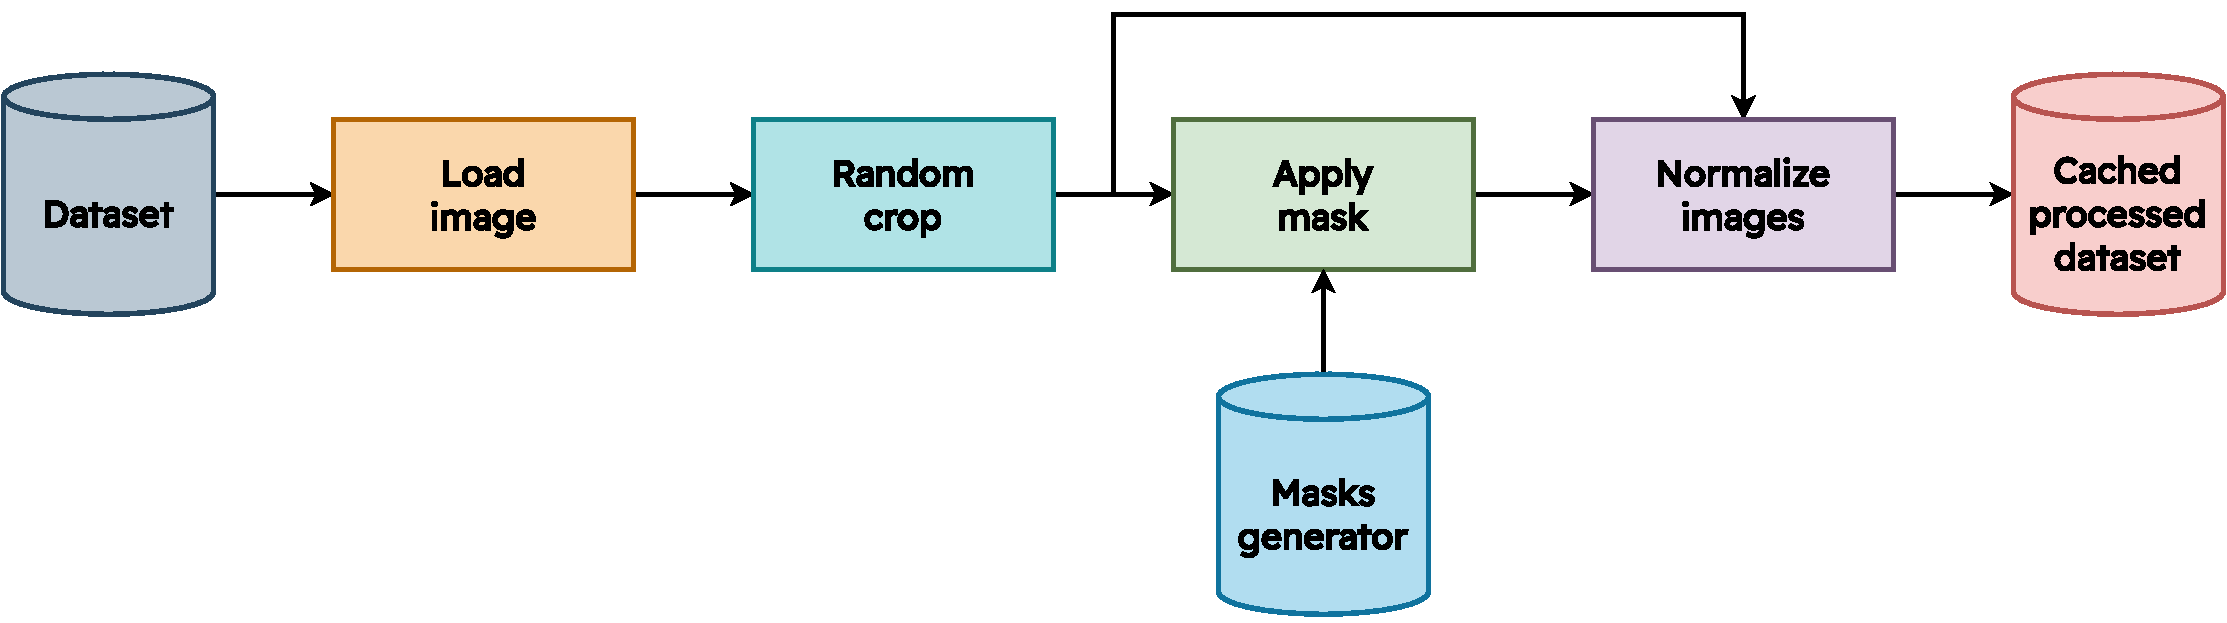
\includegraphics[width=0.86\textwidth]{state-of-the-art/pipeline.pdf}
    \caption[Coarse inpainting network followed by a refinement network architecture]{Coarse inpainting network followed by a refinement network architecture~\supercite{free-form-inpainting}}
    \label{fig:pipeline}
\end{figure}

\begin{figure}[ht]
    \centering
    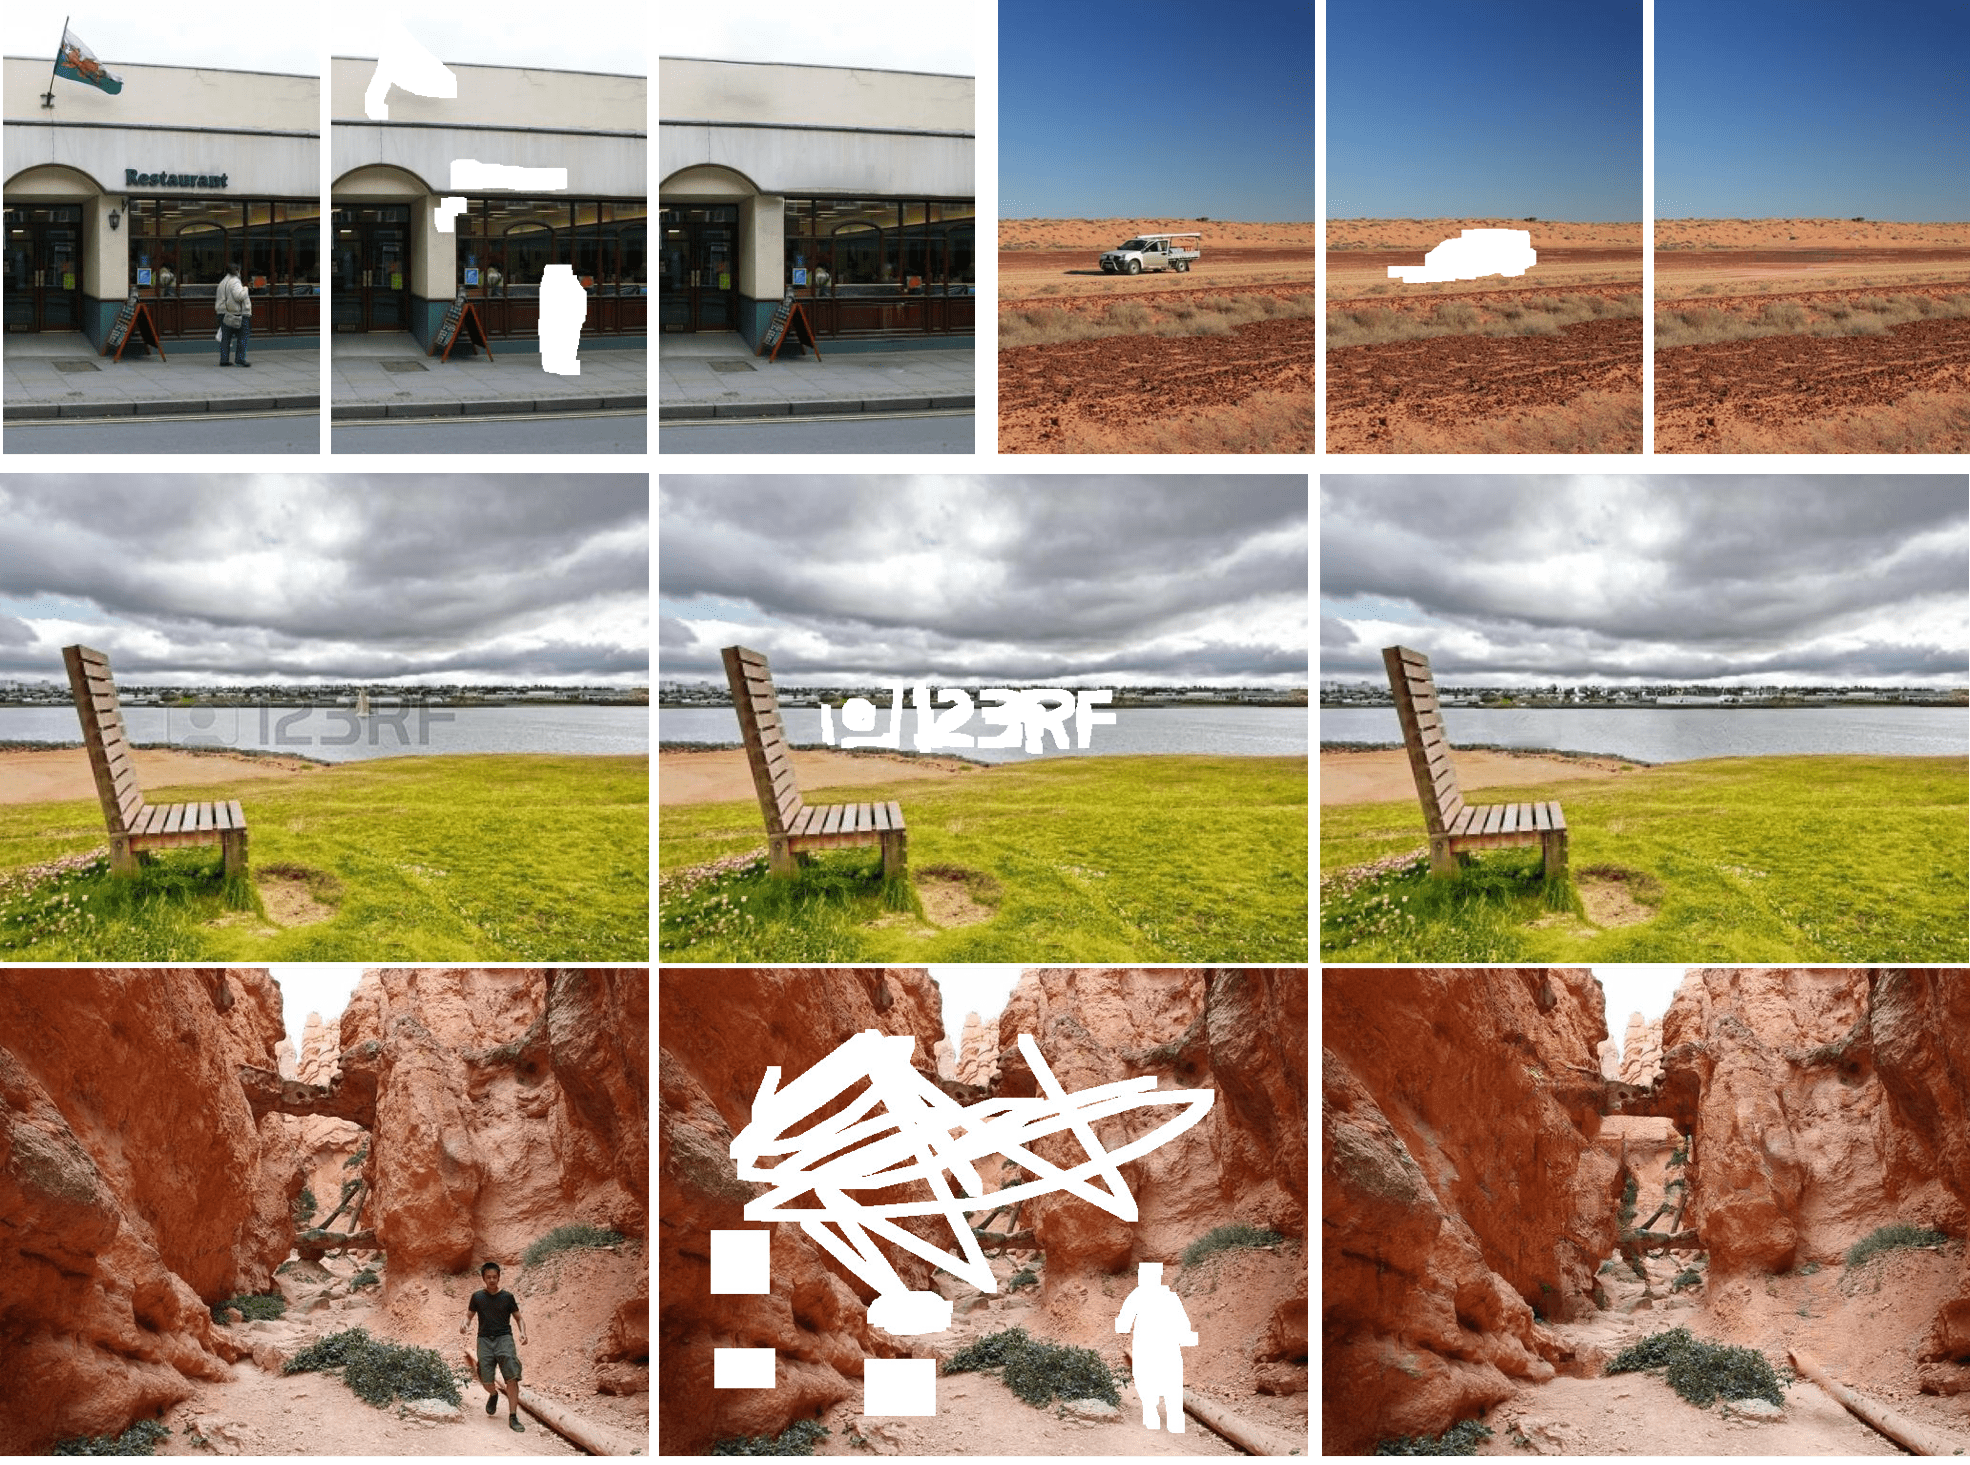
\includegraphics[width=0.95\textwidth]{state-of-the-art/example1.png}
    \caption[Inpainting example using the Free-Form architecture]{Inpainting example using the Free-Form architecture\supercite{free-form-inpainting}}
    \label{fig:example1}
\end{figure}

\begin{figure}[ht]
    \centering
    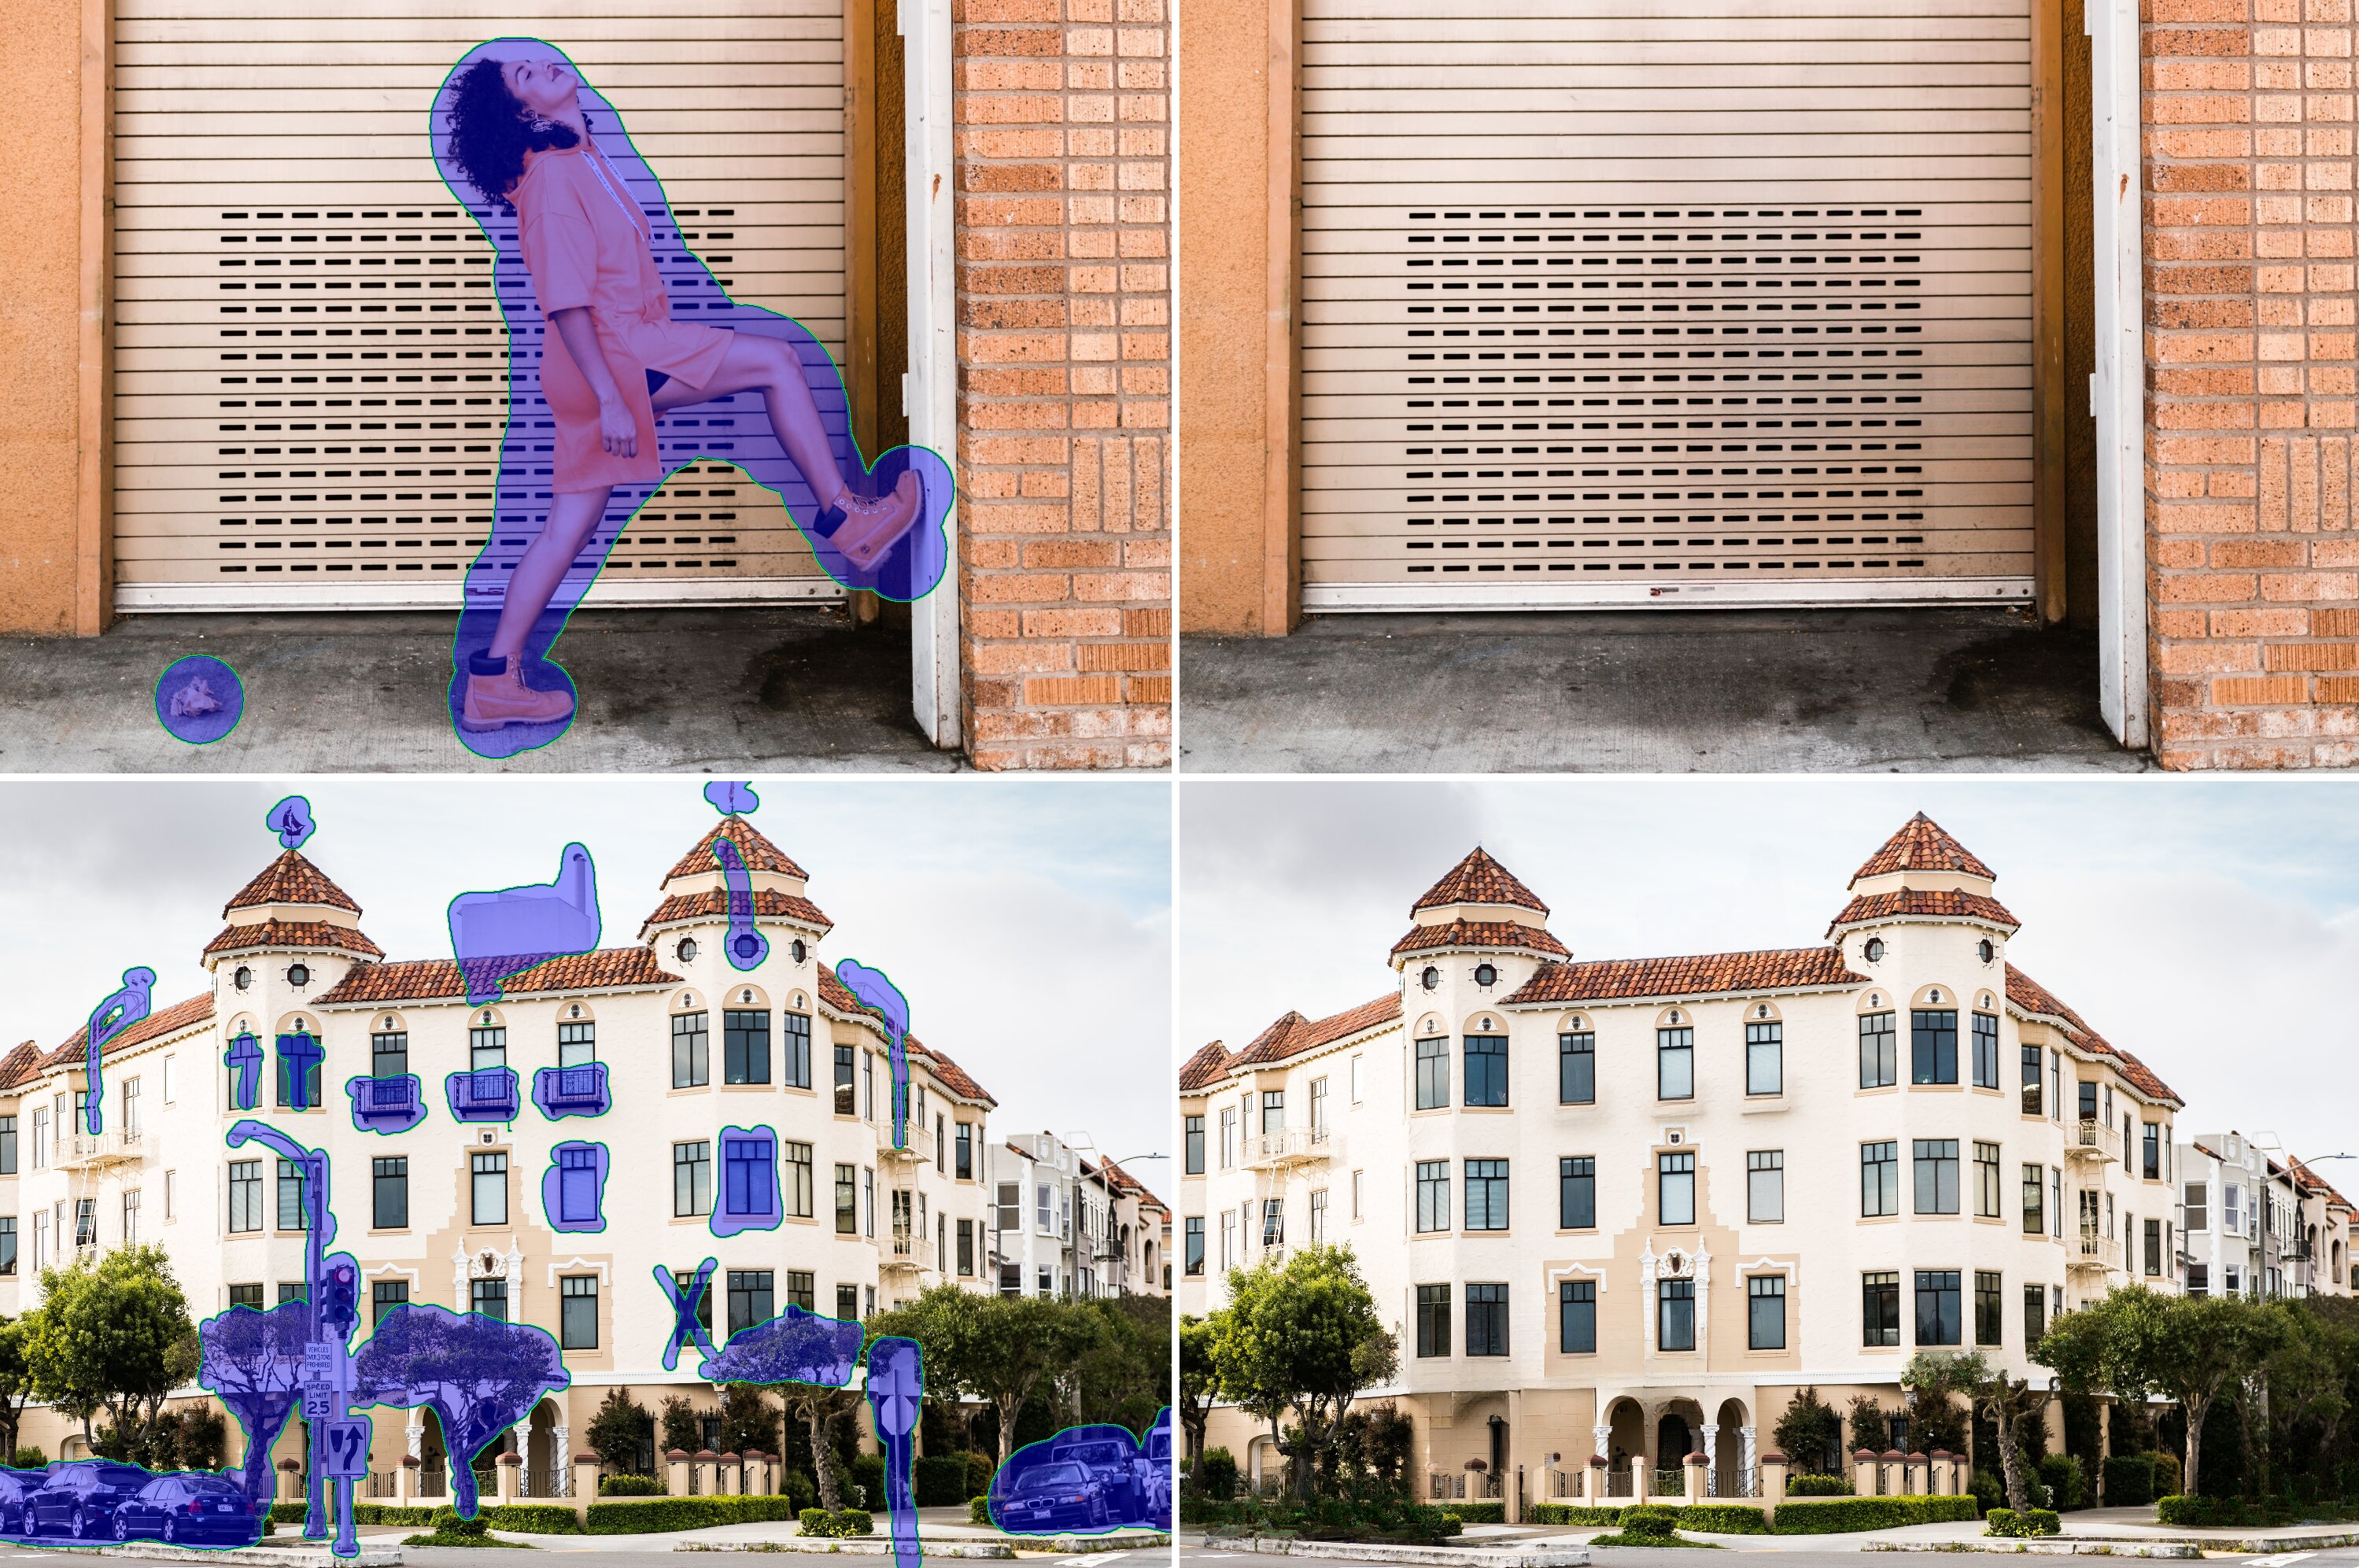
\includegraphics[width=0.95\textwidth]{state-of-the-art/example2.jpg}
    \caption[Inpainting example using the Fourier Convolutions architecture]{Inpainting example using the Fourier Convolutions architecture~\supercite{fourier-conv}}
    \label{fig:example2}
\end{figure}
